\documentclass[tikz,border=10pt]{standalone}
% No TikZ libraries needed: only basic drawing and nodes are used.
\begin{document}
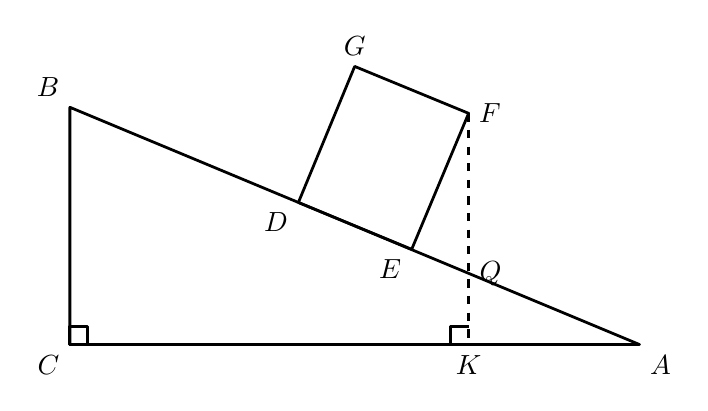
\begin{tikzpicture}[line join=round, line width=1.0pt, font=\fontsize{10}{12}\selectfont]
  % Scale s = 0.008511 cm/px; origin at C; y flipped (y_t = (514 - py) * s)
  \coordinate (A) at (7.234,0);
  \coordinate (B) at (0,3.013);
  \coordinate (C) at (0,0);
  \coordinate (K) at (5.064,0);
  \coordinate (D) at (2.902,1.804);
  \coordinate (E) at (4.341,1.209);
  \coordinate (F) at (5.064,2.936);
  \coordinate (G) at (3.617,3.532);
  \coordinate (Q) at (5.068,0.902);

  % Solid triangle B-C-A (hypotenuse BA passes through D, E, Q)
  \draw (B) -- (C) -- (A) -- cycle;

  % Solid quadrilateral D-E-F-G (DE lies on BA)
  \draw (D) -- (E) -- (F) -- (G) -- cycle;

  % Dashed vertical segment F to K
  \draw[dashed] (F) -- (K);

  % Right-angle mark at C: full square from the vertex, side 0.226 cm (26.6 px)
  \draw (0,0) -- (0.226,0) -- (0.226,0.226) -- (0,0.226) -- cycle;

  % Right-angle mark at K (inside triangle corner, toward F)
  \draw (4.838,0) -- (4.838,0.226) -- (5.064,0.226);

  % Labels
  \node[above left]  at (B) {$B$};
  \node[below left]  at (C) {$C$};
  \node[below right] at (A) {$A$};
  \node[below]       at (K) {$K$};
  \node[below left]  at (D) {$D$};
  \node[below left]  at (E) {$E$};
  \node[right]       at (F) {$F$};
  \node[above]       at (G) {$G$};
  \node[right]       at (Q) {$Q$};
\end{tikzpicture}
\end{document}